\documentclass{beamer}
\usepackage{up}

\title{Рекурсия}

\date{14 декември 2016 г.}

\usetikzlibrary{arrows.meta}

\begin{document}

\begin{frame}
  \titlepage
\end{frame}

\section{Какво е рекурсия?}

\begin{frame}<1-4>
  \frametitle{Какво е рекурсия?}
  
  \begin{center}
    \temporal<2>{
      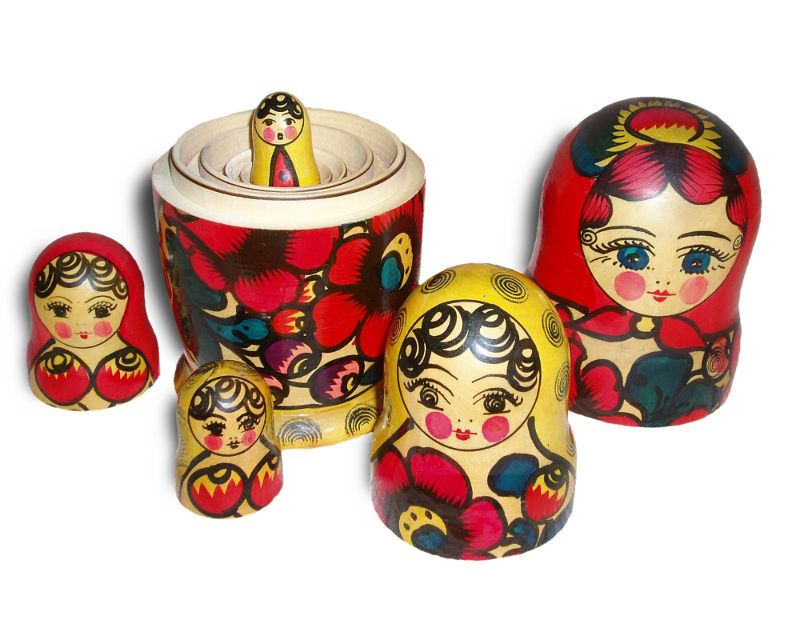
\includegraphics[width=.8\textwidth]{images/matroska.jpg}
    }{
      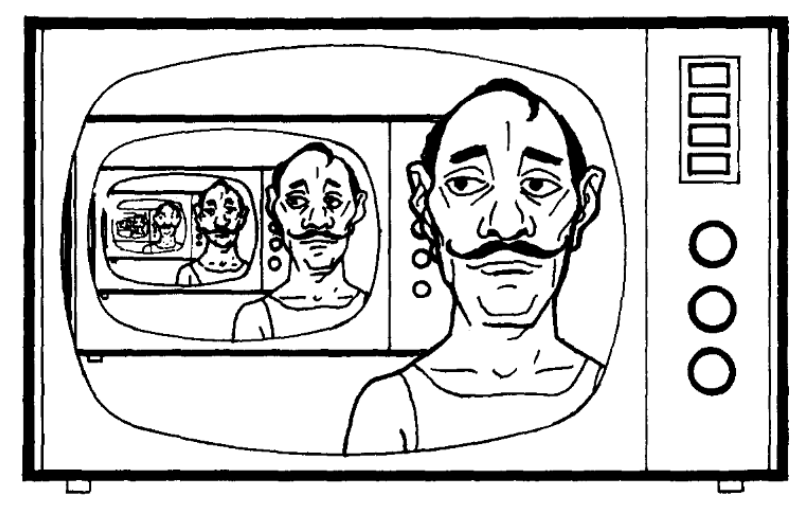
\includegraphics[width=.8\textwidth]{images/knuth.png}
    }{ \only<3>{
        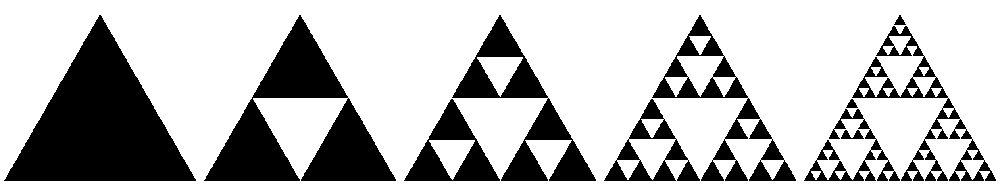
\includegraphics[width=.8\textwidth]{images/sierpinski.png}
      }}
  \end{center}
  \begin{itemize}[<+(4)->]
  \item Повторени чрез позоваване на себе си
  \item ``приятелите на моите приятели са и мои приятели''
  \item директориите съдържат файлове и директории
  \item PHP = PHP Hypertext preprocessor
  \item за да строшите камък:
    \begin{itemize}
    \item ударете с чука, за да натрошите камъка на части
    \item строшете получените по-малки камъни
    \end{itemize}
  \item за разберете какво е рекурсия, трябва да разберете какво е рекурсия
  \end{itemize}
\end{frame}

\begin{frame}
  \frametitle{Рекурсията в математиката}

  \begin{equation*}
    n! =
    \begin{cases}
      1,& n = 0,\\
      n(n-1)!,&n > 0.
    \end{cases}
  \end{equation*}
  \pause
  \begin{equation*}
    x^n =
    \begin{cases}
      1,&n = 0,\\
      x.x^{n-1},&n > 0,\\
      \frac1{x^{-n}},&n<0.
    \end{cases}
  \end{equation*}
  \pause
  \begin{equation*}
    gcd(a,b)=
    \begin{cases}
      a,&a = b,\\
      gcd(a-b,b),&a>b,\\
      gcd(a,b-a),&a<b.
    \end{cases}
  \end{equation*}
  \pause
  \begin{equation*}
    f(x)=
    \begin{cases}
      0,&x = 0,\\
      f(x+1)-1,&x>0.
    \end{cases}
  \end{equation*}
\end{frame}

\begin{frame}
  \frametitle{Как се решават задачи с рекурсия?}
  
  \begin{itemize}[<+->]
  \item \alert{Декомпозиция} --- свеждане на дадена задача към множество от по-прости задачи
  \item Рекурсията е вид декомпозиция, при който свеждаме задача към множество от по-прости задачи \alert{подобни на първоначалната}
  \item Как работи:
    \begin{itemize}
    \item Показваме решението на най-простите задачи \alert{(база, дъно)}
    \item Показваме как по-сложна задача се свежда към една или няколко по-прости \alert{(стъпка)}
    \end{itemize}
  \end{itemize}
\end{frame}

\begin{frame}
  \frametitle{Математическа индукция}

  \begin{definition}
    \textbf{Математическата индукция} е метод за доказателство, използващ като предпоставка свойството, което се доказва.
  \end{definition}
  \pause
  \textbf{Пример:} Да се докаже, че $2 + 4 + ... + 2n = n(n+1)$.
  \pause
  \textbf{Доказателство:}
  \begin{itemize}[<+->]
  \item за $n = 0$: трябва да проверим, че $0 = 0.1\quad\checkmark$
  \item нека допуснем, че сме доказали свойството за дадено $n$
  \item ще го докажем за $n+1$:
  \item $(2 + 4 + ... + 2n) + 2(n+1) = n(n+1) + 2(n+1) = (n+1)(n+2)\quad\checkmark$
  \item \textbf{Следователно:} доказахме свойството за произволно $n$. $\qed$
  \end{itemize}
  \onslide<+->
  Математическата индукция е рекурсивен метод за доказателство.
\end{frame}

\end{document}
